%% secoes/03-resultados.tex — incluído por main.tex

%%=====================================================================%%
\section{Resultados}\label{sec:resultados}
%%=====================================================================%%

A análise foi feita separadamente para cada um dos quatro desfechos: baixo peso ao nascer, nascimento pré-termo, malformação congênita e Apgar baixo no quinto minuto. 
Cada subgrupo é descrito por uma conjunção de atributos. As tabelas trazem, para cada regra: o total de nascimentos abrangidos (Total) e sua participação no total do segmento (Total \%); o número de ocorrências do desfecho no conjunto (Nº de ocorrências) e sua participação no total de ocorrências do segmento (Nº de ocorrências \%); e o lift em relação à prevalência basal do segmento.

%O total de nascimentos considerado em cada desfecho é apresentado na respectiva tabela de distribuição e serve de base para os percentuais de cada subgrupo. Para cada desfecho, os resultados de cada população são descritos em uma subseção própria, considerando apenas os subgrupos daquela população. A comparação entre as populações é feita ao final, em uma subseção de análise geral do desfecho.

%%---------------------------------------------------------------------%%
%% Subseções dos resultados, um arquivo por desfecho.                  %%
%% Caminhos relativos à pasta do manuscrito, não à deste arquivo.      %%
%%---------------------------------------------------------------------%%

%% secoes/resultados/01-baixo-peso.tex — incluído por main.tex

%%---------------------------------------------------------------------%%
\subsection{Baixo peso ao nascer}\label{subsec:res-bpn}
%%---------------------------------------------------------------------%%

A Tabela~\ref{tab:bpn-dist} mostra a distribuição do baixo peso ao nascer nas oito populações. No recorte geral, a prevalência basal do desfecho foi de 7,25\%. Cada segmento tem a sua própria prevalência basal, indicada no título da respectiva tabela, e é sempre contra ela que se calcula o risco relativo (lift) dos subgrupos daquele segmento.

Chama atenção que cinco dos sete segmentos vulneráveis ficaram abaixo desse valor: indígena (6,16\%), rural (6,40\%), beneficiárias do Bolsa Família (6,54\%), quilombola (6,74\%) e municípios de até 10 mil habitantes (6,90\%). Apenas dois ficaram acima: mães com baixa escolaridade (7,90\%) e mães com menos de 15 anos (11,60\%).

\begin{table}[htbp]
\caption{Distribuição do baixo peso ao nascer por população analisada.}\label{tab:bpn-dist}%
\begin{tabularx}{\textwidth}{@{}Yrrrr@{}}
\toprule
População & Total & \makecell{Total\\(\%)} & \makecell{Nº de\\ocorrências} & \makecell{Ocorrências\\(\%)}\\
\midrule
Recorte geral & 5.242.215 & 100,00 & 380.321 & 7,25\\
Municípios até 10 mil hab. & 427.215 & 8,15 & 29.466 & 6,90\\
Rural & 1.129.845 & 21,55 & 72.315 & 6,40\\
Indígena & 46.150 & 0,88 & 2.843 & 6,16\\
Quilombola & 25.508 & 0,49 & 1.719 & 6,74\\
Mães com baixa escolaridade & 209.182 & 3,99 & 16.529 & 7,90\\
Mães menores de 15 anos & 26.652 & 0,51 & 3.091 & 11,60\\
Beneficiárias do Bolsa Família & 1.221.833 & 23,31 & 79.942 & 6,54\\
\bottomrule
\end{tabularx}
%\fontetabela
\end{table}


A Tabela~\ref{tab:bpn} apresenta os cinco subgrupos mais de maior WRAcc para o baixo peso ao nascer considerando os oito recortes deste estudo.
Como pode ser observado, alguns itens se repetem como marcadores de risco de baixo peso, com intensidades distintas entre os recortes. O número de consultas de pré-natal é o item mais recorrente, presente em 23 dos 40 subgrupos e em todos os recortes. Isolada, a faixa de 1 a 3 consultas varia de 24\% acima da basal na população indígena a 87\% entre mães com menos de 15 anos, passando por 66\% no recorte geral, e é o subgrupo de maior risco da tabela no recorte geral, entre mães com baixa escolaridade e entre beneficiárias do Bolsa Família. As regras com a faixa de 4 a 6 consultas que não incluem a primeira gestação ficam entre 20\% e 46\% acima da basal, com exceção do subgrupo 8 dos municípios de até 10 mil habitantes (57\%).
 

\begin{table}[p] % [p] coloca a tabela grande em uma página dedicada, evitando quebrar o fluxo do texto
\centering
\caption{Subgrupos baixo peso ao nascer (prevalência basal: 7,25\%).}
\label{tab:bpn}

% Ajustes para caber em uma única página com legibilidade clínica/epidemiológica
\scriptsize % Fonte padrão para tabelas densas em periódicos de saúde
\setlength{\tabcolsep}{4pt} % Reduz margem lateral interna das células (padrão é 6pt)
\renewcommand{\arraystretch}{1.08} % Compacta levemente a altura das linhas sem esmagar o texto

\begin{tabularx}{\textwidth}{@{}c Y r r r r r@{}}
\toprule
\textbf{\#} & \textbf{Subgrupo} & \textbf{Total} & \textbf{\makecell[r]{Total\\(\%)}} & \textbf{\makecell[r]{Nº de\\ocorr.}} & \textbf{\makecell[r]{Ocorr.\\(\%)}} & \textbf{Lift} \\
\midrule
\secaotabela{Recorte geral}
1 & nascimento hospitalar; consultas: 4--6 & 1.609.468 & 30,7 & 144.933 & 38,1 & 1,24 \\
2 & destino do lixo: coletado; sexo: F & 1.941.005 & 37,0 & 162.198 & 42,6 & 1,15 \\
3 & consultas: 1--3 & 427.185 & 8,1 & 51.522 & 13,5 & 1,66 \\
4 & escoamento sanitário: rede coletora; consultas: 4--6 & 606.962 & 11,6 & 64.446 & 16,9 & 1,46 \\
5 & água canalizada: sim; sexo: F; consultas: 4--6 & 604.665 & 11,5 & 62.542 & 16,4 & 1,43 \\

\secaotabela{Municípios de até 10 mil habitantes}
6 & consultas: 4--6 & 121.922 & 28,5 & 11.137 & 37,8 & 1,32 \\
7 & sexo: F & 208.607 & 48,8 & 16.217 & 55,0 & 1,13 \\
8 & consultas: 4--6; início do pré-natal: 1--3; Bolsa Família: não & 44.649 & 10,5 & 4.849 & 16,5 & 1,57 \\
9 & primeira gestação: sim & 119.156 & 27,9 & 9.814 & 33,3 & 1,19 \\
10 & primeira gestação: sim; consultas: 4--6 & 31.344 & 7,3 & 3.754 & 12,7 & 1,74 \\

\secaotabela{População rural}
11 & nascimento hospitalar; consultas: 4--6 & 374.735 & 33,2 & 28.818 & 39,9 & 1,20 \\
12 & primeira gestação: sim & 276.899 & 24,5 & 22.404 & 31,0 & 1,26 \\
13 & sexo: F & 552.138 & 48,9 & 39.698 & 54,9 & 1,12 \\
14 & primeira gestação: sim; consultas: 4--6 & 89.166 & 7,9 & 9.620 & 13,3 & 1,69 \\
15 & consultas: 1--3 & 112.897 & 10,0 & 10.701 & 14,8 & 1,48 \\

\secaotabela{População indígena}
16 & primeira gestação: sim & 8.489 & 18,4 & 734 & 25,8 & 1,40 \\
17 & sexo: F & 22.546 & 48,9 & 1.584 & 55,7 & 1,14 \\
18 & despesa com aluguel: 0; idade materna menor que 20 anos & 9.549 & 20,7 & 769 & 27,0 & 1,31 \\
19 & consultas: 1--3 & 9.933 & 21,5 & 758 & 26,7 & 1,24 \\
20 & sexo: F; mãe solteira & 8.922 & 19,3 & 694 & 24,4 & 1,26 \\

\secaotabela{População quilombola}
21 & primeira gestação: sim & 5.924 & 23,2 & 536 & 31,2 & 1,34 \\
22 & nascimento hospitalar; consultas: 1--3 & 2.902 & 11,4 & 305 & 17,7 & 1,56 \\
23 & primeira gestação: sim; consultas: 4--6 & 2.188 & 8,6 & 243 & 14,1 & 1,65 \\
24 & idade materna menor que 20 anos & 5.299 & 20,8 & 449 & 26,1 & 1,26 \\
25 & despesa com transporte: 0; Bolsa Família: não & 10.951 & 42,9 & 818 & 47,6 & 1,11 \\

\secaotabela{Mãe com baixa escolaridade}
26 & consultas: 1--3 & 28.030 & 13,4 & 3.259 & 19,7 & 1,47 \\
27 & primeira gestação: sim & 47.950 & 22,9 & 4.732 & 28,6 & 1,25 \\
28 & sexo: F & 102.821 & 49,2 & 9.055 & 54,8 & 1,11 \\
29 & consultas: 4--6; material do domicílio: tijolo/alvenaria & 49.452 & 23,6 & 4.737 & 28,7 & 1,21 \\
30 & consultas: 4--6; sexo: F & 37.176 & 17,8 & 3.708 & 22,4 & 1,26 \\

\secaotabela{Mãe com menos de 15 anos}
31 & consultas: 1--3 & 3.083 & 11,6 & 670 & 21,7 & 1,87 \\
32 & parto normal & 15.516 & 58,2 & 2.051 & 66,4 & 1,14 \\
33 & parto normal; consultas: 4--6 & 6.091 & 22,9 & 887 & 28,7 & 1,26 \\
34 & mãe solteira; parto normal; consultas: 1--3; idade materna menor que 20 anos; primeira gestação: sim & 1.178 & 4,4 & 310 & 10,0 & 2,27 \\
35 & despesa com gás de 45 ou mais; parto normal & 5.288 & 19,8 & 776 & 25,1 & 1,27 \\

\secaotabela{Beneficiário do Programa Bolsa Família}
36 & consultas: 4--6 & 388.589 & 31,8 & 31.209 & 39,0 & 1,23 \\
37 & sexo: F & 599.793 & 49,1 & 43.913 & 54,9 & 1,12 \\
38 & consultas: 1--3 & 92.550 & 7,6 & 10.359 & 13,0 & 1,71 \\
39 & consultas: 4--6; parto cesárea & 153.193 & 12,5 & 13.982 & 17,5 & 1,39 \\
40 & consultas: 4--6; sexo: F; destino do lixo: coletado & 126.825 & 10,4 & 12.141 & 15,2 & 1,46 \\
\bottomrule
\end{tabularx}
%\fontetabela
\end{table}


%geral
%No recorte geral (Tabela~\ref{tab:bpn}), o número de consultas de pré-natal está presente em quatro dos cinco subgrupos, em três deles na faixa de 4 a 6 consultas (subgrupos 1, 4 e 5) e em um na faixa de 1 a 3 (subgrupo 3). O sexo feminino aparece em dois subgrupos (2 e 5), e os demais itens ocorrem uma vez cada.

%O subgrupo 3 (Tabela~\ref{tab:bpn}), definido apenas por 1 a 3 consultas, apresenta o maior risco do desfecho da tabela, 66\% acima da basal do segmento, e a menor participação nas ocorrências (13,5\%). No extremo oposto, o subgrupo 2 registra o menor risco do desfecho (15\% acima da basal) e a maior participação nas ocorrências (42,6\%). Os subgrupos 4 e 5, ambos com 4 a 6 consultas somadas a itens de infraestrutura, ocupam posição intermediária, com risco 46\% e 43\% acima da basal.

%Como as regras são conjunções de atributos, esses riscos relativos não isolam o efeito de nenhum item individual. A comparação entre os subgrupos 1, 4 e 5, que compartilham a faixa de 4 a 6 consultas mas diferem nos demais itens, mostra risco 24\%, 46\% e 43\% acima da basal, o que indica que parte da variação decorre dos itens acompanhantes.

%Três dos cinco subgrupos incluem itens que descrevem condições de infraestrutura domiciliar presentes: coleta de lixo (subgrupo 2), escoamento por rede coletora (subgrupo 4) e água canalizada (subgrupo 5).

%municipios até 10k
%Já no recorte dos municípios de até 10 mil habitantes, o número de consultas aparece em três, sempre na faixa de 4 a 6, e a faixa de 1 a 3 não figura entre os cinco primeiros. A primeira gestação aparece em dois subgrupos (9 e 10).

%O subgrupo 10 apresenta o maior risco do desfecho da tabela, 74\% acima da basal, e a menor participação nas ocorrências (12,7\%); o subgrupo 7, definido apenas pelo sexo feminino, tem o menor risco do desfecho (13\% acima da basal) e a maior participação nas ocorrências (55,0\%).

%Os subgrupos 9 e 10 permitem uma comparação com apenas um item de diferença: o subgrupo 9 é definido somente por primeira gestação e está 19\% acima da basal; o subgrupo 10 acrescenta a faixa de 4 a 6 consultas e chega a 74\% acima da basal. A participação nas ocorrências, porém, cai de 33,3\% para 12,7\%.

%O subgrupo 8 combina a faixa de 4 a 6 consultas com início do pré-natal na categoria 1--3 e ausência de Bolsa Família, com risco 57\% acima da basal.

%Rural
%Na População rural o número de consultas aparece em três, em dois na faixa de 4 a 6 (subgrupos 11 e 14) e em um na faixa de 1 a 3 (subgrupo 15). A primeira gestação aparece em dois subgrupos (12 e 14).

%O maior risco do desfecho é o do subgrupo 14 (69\% acima da basal), que também tem a menor participação nas ocorrências (13,3\%); o menor é o do subgrupo 13, definido apenas pelo sexo feminino (12\% acima da basal), com a maior participação nas ocorrências (54,9\%).

%Assim como no segmento anterior, os subgrupos 12 e 14 diferem por um único item: a primeira gestação isolada está 26\% acima da basal, e a adição da faixa de 4 a 6 consultas eleva o risco para 69\% acima da basal, reduzindo a participação nas ocorrências de 31,0\% para 13,3\%.

%Neste segmento, a regra que contém a faixa de 1 a 3 consultas (subgrupo 15, 48\% acima da basal) apresenta risco inferior ao da regra com 4 a 6 consultas do subgrupo 14 (69\% acima da basal). Como as duas regras diferem também nos demais itens, a comparação entre as faixas não é direta.

%População indígena
%Na população indígena o sexo feminino aparece em dois subgrupos (17 e 20) e os demais itens ocorrem uma vez cada. O número de consultas figura em apenas um subgrupo, na faixa de 1 a 3 (subgrupo 19).

%O subgrupo 16, definido apenas por primeira gestação, apresenta o maior risco do desfecho da tabela (40\% acima da basal). Entre os subgrupos apresentados para todos os segmentos, esse é o maior risco observado para a regra composta unicamente por primeira gestação, acima dos 34\% do segmento quilombola e dos 26\% do rural.

%O menor risco do desfecho é o do subgrupo 17 (14\% acima da basal), que também tem a maior participação nas ocorrências (55,7\%). A menor participação nas ocorrências é a do subgrupo 20 (24,4\%), o maior valor mínimo entre os oito conjuntos analisados.

%O risco associado à faixa de 1 a 3 consultas neste segmento (24\% acima da basal) é o menor observado para essa faixa entre todos os subgrupos apresentados.

%Quilombora
%Na População quilombola a primeira gestação aparece em dois subgrupos (21 e 23) e o número de consultas também em dois (subgrupos 22 e 23), em faixas distintas. Os demais itens ocorrem uma vez cada.

%O subgrupo 23 apresenta o maior risco do desfecho (65\% acima da basal) e a menor participação nas ocorrências (14,1\%) da tabela. O subgrupo 25 tem o menor risco do desfecho (11\% acima da basal) e a maior participação nas ocorrências (47,6\%).

%Os subgrupos 21 e 23 diferem por um item: a primeira gestação isolada está 34\% acima da basal, e a adição da faixa de 4 a 6 consultas eleva o risco para 65\% acima da basal, com queda da participação nas ocorrências de 31,2\% para 14,1\%.

%Neste segmento, a regra com 4 a 6 consultas (subgrupo 23, 65\% acima da basal) apresenta risco superior ao da regra com 1 a 3 consultas (subgrupo 22, 56\% acima da basal). Como os itens acompanhantes diferem entre as duas regras, a comparação entre as faixas não é direta.

%Mães com baixa escolaridade
%Nas mães com baixa escolaridade, o número de consultas aparece em três, em um na faixa de 1 a 3 (subgrupo 26) e em dois na faixa de 4 a 6 (subgrupos 29 e 30). O sexo feminino aparece em dois subgrupos (28 e 30).

%O subgrupo 26, definido apenas pela faixa de 1 a 3 consultas, tem o maior risco do desfecho (47\% acima da basal) e a menor participação nas ocorrências (19,7\%). O subgrupo 28 tem o menor risco do desfecho (11\% acima da basal) e a maior participação nas ocorrências (54,8\%).

%As regras com 4 a 6 consultas apresentam risco 21\% e 26\% acima da basal, inferior ao da regra com 1 a 3 consultas (47\%).

%Nas mães menores de 15 anos o parto normal aparece em quatro dos cinco subgrupos (32, 33, 34 e 35) e o número de consultas em três (31, 33 e 34). Este é também o segmento com o maior baixo peso ao nascer entre os oito analisados (Tabela~\ref{tab:bpn-dist}).

%O subgrupo 34 apresenta o maior risco entre todos os subgrupos do baixo peso ao nascer (127\% acima da basal, isto é, 2,27 vezes a basal), com a menor participação nas ocorrências da tabela (10,0\%). 
%Trata-se de uma conjunção de cinco itens: mãe solteira, parto normal, 1 a 3 consultas, idade inferior a 20 anos e primeira gestação. 
%O item relativo à idade é redundante dentro de um segmento composto por mães com menos de 15 anos.

%O subgrupo 31, definido apenas pela faixa de 1 a 3 consultas, está 87\% acima da basal, o maior valor observado para essa faixa isolada entre todos os segmentos. O subgrupo 32, definido apenas por parto normal, tem o menor risco do desfecho (14\% acima da basal) e a maior participação nas ocorrências de toda a análise (66,4\%).

%As regras com 4 a 6 consultas apresentam risco 26\% acima da basal, inferior ao das regras com 1 a 3 consultas (87\% e 127\%).

%Por fim, nos beneficiárias do Bolsa Família o número de consultas aparece em quatro dos cinco subgrupos, em três na faixa de 4 a 6 (36, 39 e 40) e em um na faixa de 1 a 3 (subgrupo 38), e o sexo feminino aparece em dois (37 e 40). Este é também o segmento com o maior número de nascimentos (1.221.833).

%O subgrupo 38 tem o maior risco do desfecho (71\% acima da basal) e a menor participação nas ocorrências (13,0\%); o subgrupo 37 tem o menor risco do desfecho (12\% acima da basal) e a maior participação nas ocorrências (54,9\%). As regras com 4 a 6 consultas apresentam risco 23\%, 39\% e 46\% acima da basal, todos inferiores ao da regra com 1 a 3 consultas.

%O conjunto de itens que compõem os cinco subgrupos coincide parcialmente com o observado no recorte geral, onde também figuram o número de consultas, o sexo feminino e a coleta de lixo.
 
%Reunidos os oito recortes, alguns itens se repetem como marcadores de risco de baixo peso, com intensidades distintas entre os recortes. O número de consultas de pré-natal é o item mais recorrente, presente em 23 dos 40 subgrupos e em todos os recortes. Isolada, a faixa de 1 a 3 consultas varia de 24\% acima da basal na população indígena a 87\% entre mães com menos de 15 anos, passando por 66\% no recorte geral, e é o subgrupo de maior risco da tabela no recorte geral, entre mães com baixa escolaridade e entre beneficiárias do Bolsa Família. As regras com a faixa de 4 a 6 consultas que não incluem a primeira gestação ficam entre 20\% e 46\% acima da basal, com exceção do subgrupo 8 dos municípios de até 10 mil habitantes (57\%).
 
%subgrupos. Isolada, seu risco cresce de 19\% acima da basal nos municípios de até 10 mil habitantes para 25\% entre mães com baixa escolaridade, 26\% na população rural, 34\% na quilombola e 40\% na indígena, o maior valor dessa regra entre todos os recortes. Combinada à faixa de 4 a 6 consultas, ela forma o subgrupo de maior risco de três recortes: 74\% nos municípios pequenos, 69\% no rural e 65\% no quilombola.
 
O sexo feminino aparece em seis dos oito recortes, ausente apenas na população quilombola e entre mães menores de 15 anos. Isolado, define um subgrupo em cinco recortes (municípios de até 10 mil habitantes, rural, indígena, mães com baixa escolaridade e beneficiárias do Bolsa Família) e, em todos eles, é o subgrupo de menor risco da tabela (entre 11\% e 14\% acima da basal) e de maior cobertura (cerca de 49\% dos nascimentos e 55\% das ocorrências). No recorte geral, combinado à coleta de lixo, ocupa a mesma posição (15\% acima da basal e 37,0\% dos nascimentos). Quando acompanhado de outros itens, o risco é maior: 26\% com mãe solteira na população indígena, 26\% com 4 a 6 consultas entre mães com baixa escolaridade, e 43\% e 46\% com 4 a 6 consultas e itens de infraestrutura no recorte geral e entre beneficiárias do Bolsa Família.
 
Os extremos estão em dois recortes. Entre as mães com menos de 15 anos, segmento de maior prevalência basal (11,60\%), está o subgrupo de maior risco do desfecho (mãe solteira, parto normal, 1 a 3 consultas e primeira gestação, 127\% acima da basal, ou 2,27 vezes), além do maior risco isolado da faixa de 1 a 3 consultas (87\%) e da maior participação de uma única regra nas ocorrências (parto normal, com 66,4\% das ocorrências). No extremo oposto, a população indígena tem o menor risco máximo entre os oito recortes (40\% acima da basal) e o menor valor da faixa de 1 a 3 consultas (24\%); é também o recorte em que a menor participação nas ocorrências é a mais alta entre os oito (24,4\%).

\FloatBarrier

%% secoes/resultados/02-pre-termo.tex — incluído por main.tex

%%---------------------------------------------------------------------%%
\subsection{Nascimento pré-termo}\label{subsec:res-pt}
%%---------------------------------------------------------------------%%

A Tabela~\ref{tab:pt-dist} mostra a distribuição do nascimento pré-termo nas oito populações. No recorte geral, a prevalência basal do desfecho foi de 10,83\%, bem acima da observada para o baixo peso ao nascer (7,25\%).

Diferentemente do que se viu no baixo peso ao nascer, aqui as maiores prevalências recaem sobre os segmentos socialmente mais vulneráveis: mães menores de 15 anos (17,26\%) e população indígena (15,43\%) apresentam os dois maiores valores, seguidas por mães com baixa escolaridade (12,77\%) e população quilombola (11,70\%), todas acima do recorte geral. Apenas três segmentos ficaram abaixo dela, sendo eles: municípios de até 10 mil habitantes (10,43\%), população rural (10,77\%) e beneficiárias do Bolsa Família (10,80\%).

\begin{table}[H]
\caption{Distribuição do nascimento pré-termo por população analisada.}\label{tab:pt-dist}%
\begin{tabularx}{\textwidth}{@{}Yrrrr@{}}
\toprule
População & Total & \makecell{Total\\(\%)} & \makecell{Nº de\\ocorrências} & \makecell{Ocorrências\\(\%)}\\
\midrule
Recorte geral & 5.019.773 & 100,00 & 543.714 & 10,83\\
Municípios até 10 mil hab. & 412.208 & 8,21 & 43.012 & 10,43\\
Rural & 1.065.151 & 21,22 & 114.747 & 10,77\\
Indígena & 43.650 & 0,87 & 6.736 & 15,43\\
Quilombola & 23.609 & 0,47 & 2.762 & 11,70\\
Mães com baixa escolaridade & 194.533 & 3,88 & 24.843 & 12,77\\
Mães menores de 15 anos & 25.208 & 0,50 & 4.351 & 17,26\\
Beneficiárias do Bolsa Família & 1.169.568 & 23,30 & 126.355 & 10,80\\
\bottomrule
\end{tabularx}
%\fontetabela
\end{table}


A Tabela~\ref{tab:pt} apresenta os cinco subgrupos de maior WRAcc para o nascimento pré-termo nos oito recortes analisados.
Podemos observar que o número de consultas de pré-natal é o item dominante em quase toda a análise: aparece entre os cinco primeiros subgrupos dos oito segmentos e, em sete deles, define isoladamente ou acompanha a maior parte das regras. Isolada, a faixa de 1 a 3 consultas é o item de maior risco em sete dos oito segmentos, de 60\% acima da basal entre mães com baixa escolaridade a 103\% em municípios de até 10 mil habitantes, e fica sempre acima da faixa de 4 a 6 consultas isolada (entre 21\% e 46\% acima da basal). A exceção é a população indígena, em que o nascimento domiciliar isolado (47\%) supera a faixa de 1 a 3 consultas (43\%). Ainda assim, mesmo a faixa de 4 a 6 consultas eleva a prevalência acima da basal em todos os segmentos em que figura isoladamente.


\begin{table}[H]
\centering
\caption{Subgrupos para nascimento pré-termo segundo estratos populacionais (prevalência basal: 10,83\%).}
\label{tab:pt}

\scriptsize
\setlength{\tabcolsep}{4pt}
\renewcommand{\arraystretch}{1.08}

\begin{tabularx}{\textwidth}{@{}c Y r r r r r@{}}
\toprule
\textbf{\#} & \textbf{Subgrupo} & \textbf{Total} & \textbf{\makecell[r]{Total\\(\%)}} & \textbf{\makecell[r]{Nº de\\ocorr.}} & \textbf{\makecell[r]{Ocorr.\\(\%)}} & \textbf{Lift} \\
\midrule
\secaotabela{Recorte geral}
1 & consultas: 4--6 & 1.579.447 & 31,5 & 230.225 & 42,3 & 1,35 \\
2 & consultas: 1--3 & 401.528 & 8,0 & 81.460 & 15,0 & 1,87 \\
3 & consultas: 4--6; escoamento sanitário: rede coletora & 586.721 & 11,7 & 90.566 & 16,7 & 1,43 \\
4 & consultas: 4--6; primeira gestação: sim & 377.450 & 7,5 & 66.202 & 12,2 & 1,62 \\
5 & consultas: 4--6; famílias no domicílio: 1 ou menos; parto cesárea & 607.040 & 12,1 & 91.066 & 16,7 & 1,39 \\

\secaotabela{Municípios de até 10 mil habitantes}
6 & consultas: 4--6 & 117.629 & 28,5 & 17.886 & 41,6 & 1,46 \\
7 & consultas: 1--3 & 24.072 & 5,8 & 5.105 & 11,9 & 2,03 \\
8 & consultas: 4--6; primeira gestação: sim & 30.450 & 7,4 & 5.451 & 12,7 & 1,72 \\
9 & consultas: 4--6; despesa com energia: 20--56 & 43.846 & 10,6 & 6.769 & 15,7 & 1,48 \\
10 & consultas: 4--6; despesa com alimentação: 100--300 & 46.984 & 11,4 & 7.059 & 16,4 & 1,44 \\

\secaotabela{População rural}
11 & consultas: 4--6 & 375.121 & 35,2 & 52.767 & 46,0 & 1,31 \\
12 & consultas: 1--3 & 104.341 & 9,8 & 20.392 & 17,8 & 1,81 \\
13 & consultas: 4--6; primeira gestação: sim & 86.128 & 8,1 & 14.764 & 12,9 & 1,59 \\
14 & consultas: 4--6; escolaridade materna: até o 5º ano & 135.955 & 12,8 & 20.042 & 17,5 & 1,37 \\
15 & consultas: 4--6; despesa com alimentação: 0--100 & 148.332 & 13,9 & 20.867 & 18,2 & 1,31 \\

\secaotabela{População indígena}
16 & consultas: 1--3 & 9.548 & 21,9 & 2.109 & 31,3 & 1,43 \\
17 & nascimento domiciliar & 8.010 & 18,4 & 1.821 & 27,0 & 1,47 \\
18 & parto normal; mãe indígena; Bolsa Família: não & 20.171 & 46,2 & 3.485 & 51,7 & 1,12 \\
19 & consultas: 1--3; despesa com alimentação: 0--100 & 3.761 & 8,6 & 896 & 13,3 & 1,54 \\
20 & despesa com alimentação: 0--100; parto normal; mãe indígena & 9.974 & 22,8 & 1.849 & 27,4 & 1,20 \\

\secaotabela{População quilombola}
21 & consultas: 1--3 & 2.894 & 12,3 & 615 & 22,3 & 1,82 \\
22 & consultas: 4--6 & 9.424 & 39,9 & 1.335 & 48,3 & 1,21 \\
23 & consultas: 4--6; escolaridade materna: até o 5º ano & 3.338 & 14,1 & 536 & 19,4 & 1,37 \\
24 & consultas: 1--3; escolaridade materna: até o 5º ano & 1.156 & 4,9 & 277 & 10,0 & 2,05 \\
25 & parto normal; escolaridade materna: até o 5º ano & 5.595 & 23,7 & 791 & 28,6 & 1,21 \\

\secaotabela{Mães com baixa escolaridade}
26 & consultas: 4--6 & 71.814 & 36,9 & 11.195 & 45,1 & 1,22 \\
27 & consultas: 1--3 & 25.484 & 13,1 & 5.214 & 21,0 & 1,60 \\
28 & consultas: 4--6; idade materna menor que 20 anos & 20.486 & 10,5 & 3.877 & 15,6 & 1,48 \\
29 & domicílio particular permanente; idade materna menor que 20 anos & 52.109 & 26,8 & 7.665 & 30,9 & 1,15 \\
30 & consultas: 4--6; cômodos no domicílio: 5--6 & 26.247 & 13,5 & 4.204 & 16,9 & 1,25 \\

\secaotabela{Mães menores de 15 anos}
31 & consultas: 1--3 & 2.866 & 11,4 & 888 & 20,4 & 1,80 \\
32 & consultas: 4--6 & 9.662 & 38,3 & 2.034 & 46,7 & 1,22 \\
33 & parto normal; primeira gestação: sim & 10.801 & 42,8 & 2.169 & 49,9 & 1,16 \\
34 & consultas: 4--6; parentesco: neto(a); parto normal & 3.693 & 14,7 & 889 & 20,4 & 1,39 \\
35 & consultas: 4--6; parto assistido por médico; primeira gestação: sim & 3.385 & 13,4 & 789 & 18,1 & 1,35 \\

\secaotabela{Beneficiárias do Programa Bolsa Família}
36 & consultas: 4--6 & 372.685 & 31,9 & 53.581 & 42,4 & 1,33 \\
37 & consultas: 1--3 & 87.002 & 7,4 & 17.530 & 13,9 & 1,87 \\
38 & consultas: 4--6; calçamento do domicílio: total & 146.603 & 12,5 & 21.920 & 17,3 & 1,38 \\
39 & consultas: 4--6; parto cesárea & 146.930 & 12,6 & 21.948 & 17,4 & 1,38 \\
30 & consultas: 4--6; material do domicílio: tijolo/alvenaria; sexo: M & 141.617 & 12,1 & 21.235 & 16,8 & 1,39 \\
\bottomrule
\end{tabularx}
%\fontetabela
\end{table}


%No recorte geral, o número de consultas aparece nos cinco subgrupos, em quatro na faixa de 4 a 6 (subgrupos 1, 3, 4 e 5) e em um na faixa de 1 a 3 (subgrupo 2). Os demais itens ocorrem uma vez cada.

%O subgrupo 2, definido apenas por 1 a 3 consultas, apresenta o maior risco do desfecho da tabela (87\% acima da basal). O subgrupo 1, definido apenas por 4 a 6 consultas, tem o menor risco do desfecho (35\% acima da basal) e a maior participação nas ocorrências (42,3\%); a menor participação nas ocorrências é a do subgrupo 4 (12,2\%).

%Os subgrupos 1, 3, 4 e 5 compartilham a faixa de 4 a 6 consultas e diferem nos demais itens, com risco 35\%, 43\%, 62\% e 39\% acima da basal. A comparação entre os subgrupos 1 e 4, que diferem pela adição da primeira gestação, mostra o risco passando de 35\% para 62\% acima da basal e a prevalência de 14,58\% para 17,54\%, com queda da participação nas ocorrências de 42,3\% para 12,2\%.

%10k
%Nos municípios de até 10 mil habitantes o número de consultas aparece nos cinco subgrupos, na faixa de 4 a 6 em quatro (6, 8, 9 e 10) e na faixa de 1 a 3 em um (subgrupo 7). A primeira gestação figura no subgrupo 8 e itens de despesa domiciliar nos subgrupos 9 e 10.

%O subgrupo 7, definido apenas por 1 a 3 consultas, apresenta o maior risco entre as regras de um único item de todo o pré-termo (103\% acima da basal) e a menor participação nas ocorrências da tabela (11,9\%). O subgrupo 6, definido apenas por 4 a 6 consultas, tem a maior participação nas ocorrências (41,6\%). Fora do subgrupo 7, o risco varia pouco, entre 44\% e 72\% acima da basal.

%Os subgrupos 6 e 8 diferem pela adição da primeira gestação, que eleva a prevalência de 15,21\% para 17,90\%, de 46\% para 72\% acima da basal, com queda da participação nas ocorrências de 41,6\% para 12,7\%.

%Rural
%Na população rural o número de consultas aparece nos cinco subgrupos, na faixa de 4 a 6 em quatro (11, 13, 14 e 15) e na faixa de 1 a 3 em um (subgrupo 12). Escolaridade materna, primeira gestação e despesa com alimentação acompanham a faixa de 4 a 6 em três subgrupos.

%O subgrupo 12 (1 a 3 consultas) apresenta o maior risco do desfecho (81\% acima da basal); os subgrupos 11 e 15 apresentam o menor (31\% acima da basal), e o subgrupo 11 tem a maior participação nas ocorrências da tabela (46,0\%).

%Os subgrupos 11 e 13 diferem pela adição da primeira gestação, que eleva a prevalência de 14,07\% para 17,14\%, de 31\% para 59\% acima da basal, reduzindo a participação nas ocorrências de 46,0\% para 12,9\%.

%indígena
%A população indígena é o único segmento em que o número de consultas não domina os cinco primeiros subgrupos: aparece em dois deles, ambos na faixa de 1 a 3 (subgrupos 16 e 19). Os demais são definidos por nascimento domiciliar (2), pela conjunção de parto normal, mãe indígena e ausência de Bolsa Família (3) e por despesa com alimentação combinada a parto normal e mãe indígena (5).

%O subgrupo 4 (16 a 18 consultas somadas a despesa com alimentação) apresenta o maior risco do desfecho da tabela (54\% acima da basal). O subgrupo 18 tem o menor risco do desfecho (12\% acima da basal) e, ao mesmo tempo, a maior participação nas ocorrências de toda a análise (51,7\%), abrangendo mais da metade dos casos do segmento.

%O risco associado à faixa de 1 a 3 consultas neste segmento (43\% acima da basal, subgrupo 16) é o menor observado para essa faixa entre todos os segmentos, assim como já ocorrera no baixo peso ao nascer.

%Na população quilombola o número de consultas aparece em quatro dos cinco subgrupos (21, 22, 23 e 24), em faixas distintas; a escolaridade materna acompanha três regras (23, 24 e 25).

%O subgrupo 24 (1 a 3 consultas somadas à escolaridade materna até o 5º ano) apresenta o maior risco do desfecho entre todos os subgrupos apresentados neste estudo para o pré-termo (105\% acima da basal), com prevalência de 23,96\%, e a menor participação nas ocorrências de todos os conjuntos (10,0\%). O subgrupo 22 (4 a 6 consultas) tem o menor risco do desfecho (21\% acima da basal), compartilhada com o subgrupo 25, e a maior participação nas ocorrências da tabela (48,3\%).

%As duas comparações de item único reforçam o efeito da escolaridade: sobre a faixa de 1 a 3 consultas, sua adição eleva o risco acima da basal de 82\% (subgrupo 21) para 105\% (subgrupo 4); sobre a faixa de 4 a 6, de 21\% (subgrupo 22) para 37\% (subgrupo 23).

%Nas mães com baixa escolaridade o número de consultas aparece em quatro dos cinco subgrupos (26, 27, 28 e 30), na faixa de 4 a 6 em três (26, 28 e 30) e na faixa de 1 a 3 em um (subgrupo 27). A idade materna inferior a 20 anos figura em dois subgrupos (28 e 29).

%O subgrupo 27 (1 a 3 consultas) apresenta o maior risco do desfecho (60\% acima da basal); o subgrupo 29, único dos cinco sem o número de consultas, apresenta o menor (15\% acima da basal). A maior participação nas ocorrências é a do subgrupo 26 (45,1\%), definido apenas por 4 a 6 consultas.

%A comparação entre os subgrupos 26 e 28 mostra que a adição da idade materna inferior a 20 anos eleva a prevalência de 15,59\% para 18,93\%, de 22\% para 48\% acima da basal.

%As mães menores de 15 anos é o segmento com a maior prevalência basal entre os oito analisados (17,26\%). O número de consultas aparece em quatro dos cinco subgrupos (31, 32, 34 e 35) e o parto normal em dois (33 e 34).

%O subgrupo 31, definido apenas por 1 a 3 consultas, apresenta o maior risco do desfecho da tabela (80\% acima da basal) e a maior prevalência absoluta entre todos os subgrupos do pré-termo (30,98\%). O subgrupo 33 (parto normal e primeira gestação) tem o menor risco do desfecho (16\% acima da basal) e a maior participação nas ocorrências (49,9\%); a menor participação nas ocorrências é a do subgrupo 35 (18,1\%).

%Os subgrupos 34 e 35, que somam à faixa de 4 a 6 consultas outros itens, apresentam risco 39\% e 35\% acima da basal, superiores ao da faixa de 4 a 6 isolada (subgrupo 32, 22\%).

%Os beneficiárias do Bolsa Família é o segmento com o maior número de nascimentos (1.169.568). O número de consultas aparece nos cinco subgrupos, na faixa de 4 a 6 em quatro (36, 38, 39 e 40) e na faixa de 1 a 3 em um (subgrupo 37).

%O subgrupo 37 (1 a 3 consultas) apresenta o maior risco do desfecho (87\% acima da basal) e a menor participação nas ocorrências (13,9\%); o subgrupo 36 (4 a 6 consultas), o menor risco do desfecho (33\% acima da basal) e a maior participação nas ocorrências (42,4\%).

%Os subgrupos 38, 39 e 40 somam à faixa de 4 a 6 consultas itens de infraestrutura domiciliar e características do parto, com risco muito próximo entre si (38\%, 38\% e 39\% acima da basal) e pouco acima do subgrupo 36. O conjunto de itens coincide parcialmente com o do recorte geral, onde também figuram o número de consultas e o parto cesárea.

%Considerando os oito segmentos (Tabela˜\ref{tab:pt}), podemos observar que o número de consultas de pré-natal é o item dominante em quase toda a análise: aparece entre os cinco primeiros subgrupos dos oito segmentos e, em sete deles, define isoladamente ou acompanha a maior parte das regras. Isolada, a faixa de 1 a 3 consultas é o item de maior risco em sete dos oito segmentos, de 60\% acima da basal entre mães com baixa escolaridade a 103\% em municípios de até 10 mil habitantes, e fica sempre acima da faixa de 4 a 6 consultas isolada (entre 21\% e 46\% acima da basal). A exceção é a população indígena, em que o nascimento domiciliar isolado (47\%) supera a faixa de 1 a 3 consultas (43\%). Ainda assim, mesmo a faixa de 4 a 6 consultas eleva a prevalência acima da basal em todos os segmentos em que figura isoladamente.
 
A população indígena é a exceção, sendo o único segmento em que o número de consultas não domina os cinco primeiros subgrupos, aparecendo em apenas dois deles. O risco associado à faixa de 1 a 3 consultas nesse segmento (43\% acima da basal) é o menor observado para essa faixa entre todos os segmentos, assim como já ocorrera no baixo peso ao nascer. É também nele que está a regra com a maior participação nas ocorrências de toda a análise (subgrupo 18, com 51,7\% dos casos).
 
A regra formada apenas pela faixa de 4 a 6 consultas e pela primeira gestação aparece em três recortes e, em todos, eleva o risco em relação à faixa de 4 a 6 isolada: de 35\% para 62\% no recorte geral, de 46\% para 72\% nos municípios de até 10 mil habitantes e de 31\% para 59\% na população rural. A escolaridade materna até o 5º ano acompanha a faixa de 4 a 6 consultas na população rural (37\%) e na quilombola (37\%), e a idade materna inferior a 20 anos figura apenas entre mães com baixa escolaridade.
 
Entre as regras compostas por um único item, a faixa de 1 a 3 consultas nos municípios de até 10 mil habitantes apresenta o maior risco do pré-termo (103\% acima da basal). 
Considerando todas as regras, o maior risco relativo para o pré-termo é o do subgrupo 24 da população quilombola (1 a 3 consultas e escolaridade materna até o 5º ano, 105\% acima da basal), que também tem a menor participação nas ocorrências entre todos os conjuntos (10,0\%). Já a maior prevalência absoluta em um subgrupo está entre as mães menores de 15 anos, segmento de maior prevalência basal (17,26\%): no subgrupo definido apenas por 1 a 3 consultas, 30,98\% dos nascimentos são pré-termo, com risco 80\% acima da basal.
 
Por fim, as beneficiárias do Bolsa Família, segmento com o maior número de nascimentos (1.169.568), têm um conjunto de itens que coincide parcialmente com o do recorte geral, onde também figuram o número de consultas e o parto cesáreo.

\FloatBarrier

%% secoes/resultados/03-malformacao.tex — incluído por main.tex

%%---------------------------------------------------------------------%%
\subsection{Malformação congênita}\label{subsec:res-malf}
%%---------------------------------------------------------------------%%

A Tabela~\ref{tab:malf-dist} mostra a distribuição da malformação congênita nas oito populações. No recorte geral, a prevalência basal do desfecho foi de 0,60\%, a menor entre os quatro desfechos analisados.

As prevalências variam pouco entre os segmentos, de 0,47\% a 0,63\%. Seis dos sete segmentos vulneráveis ficaram abaixo do recorte geral: quilombola (0,47\%), indígena (0,48\%), rural (0,48\%), municípios de até 10 mil habitantes (0,54\%), mães com baixa escolaridade (0,56\%) e beneficiárias do Bolsa Família (0,56\%). Apenas as mães menores de 15 anos ficaram acima (0,63\%). Por se tratar de um desfecho raro, os segmentos menores reúnem poucas ocorrências: 227 na população indígena, 169 entre mães menores de 15 anos e 121 na população quilombola.

\begin{table}[htbp]
\caption{Distribuição da malformação congênita por população analisada.}\label{tab:malf-dist}%
\begin{tabularx}{\textwidth}{@{}Yrrrr@{}}
\toprule
População & Total & \makecell{Total\\(\%)} & \makecell{Nº de\\ocorrências} & \makecell{Ocorrências\\(\%)}\\
\midrule
Recorte geral & 5.246.679 & 100,00 & 31.270 & 0,60\\
Municípios até 10 mil hab. & 427.806 & 8,15 & 2.308 & 0,54\\
Rural & 1.133.241 & 21,60 & 5.446 & 0,48\\
Indígena & 47.474 & 0,90 & 227 & 0,48\\
Quilombola & 25.643 & 0,49 & 121 & 0,47\\
Mães com baixa escolaridade & 210.086 & 4,00 & 1.169 & 0,56\\
Mães menores de 15 anos & 26.671 & 0,51 & 169 & 0,63\\
Beneficiárias do Bolsa Família & 1.222.696 & 23,30 & 6.817 & 0,56\\
\bottomrule
\end{tabularx}
\fontetabela
\end{table}


A Tabela~\ref{tab:malf} apresenta os cinco subgrupos de maior WRAcc para a malformação congênita para os oito recortes considerados no artigo.
Na malformação congênita, dois itens aparecem nos oito recortes. O sexo masculino figura em pelo menos um subgrupo de cada recorte, e o parto cesáreo também. Em seis dos oito recortes, o subgrupo de maior risco contém o parto cesáreo: municípios de até 10 mil habitantes (31\% acima da basal), rural (47\%), indígena (71\%), quilombola (158\%), mães com baixa escolaridade (50\%) e mães menores de 15 anos (154\%). As exceções são o recorte geral e as beneficiárias do Bolsa Família, cujos subgrupos de maior risco combinam o sexo masculino a outros itens.

\begin{table}[p]
\centering
\caption{Subgrupos para malformação congênita (prevalência basal: 0,60\%).}
\label{tab:malf}

\scriptsize
\setlength{\tabcolsep}{4pt}
\renewcommand{\arraystretch}{1.04} % Levemente mais compacto para compensar subgrupos com 4-5 condições

\begin{tabularx}{\textwidth}{@{}c Y r r r r r@{}}
\toprule
\textbf{\#} & \textbf{Subgrupo} & \textbf{Total} & \textbf{\makecell[r]{Total\\(\%)}} & \textbf{\makecell[r]{Nº de\\ocorr.}} & \textbf{\makecell[r]{Ocorr.\\(\%)}} & \textbf{Lift} \\
\midrule
\secaotabela{Recorte geral}
1 & água canalizada: sim; banheiro: sim; sexo: M & 2.049.407 & 39,1 & 15.020 & 48,0 & 1,23 \\
2 & banheiro: sim; escoamento sanitário: rede coletora & 2.216.543 & 42,2 & 15.930 & 50,9 & 1,21 \\
3 & água canalizada: sim; banheiro: sim; parto cesárea & 1.947.713 & 37,1 & 14.012 & 44,8 & 1,21 \\
4 & escoamento sanitário: rede coletora; sexo: M; transferência de renda: não; Bolsa Família: não & 792.340 & 15,1 & 6.768 & 21,6 & 1,43 \\
5 & sexo: M; parto cesárea; Bolsa Família: não & 976.618 & 18,6 & 7.777 & 24,9 & 1,34 \\

\secaotabela{Municípios de até 10 mil habitantes}
6 & banheiro: sim; despesa com transporte: 0; nascimento hospitalar; parto cesárea; sabe ler e escrever: sim & 142.432 & 33,3 & 939 & 40,7 & 1,22 \\
7 & banheiro: sim; sexo: M; despesa com transporte: 0; nascimento hospitalar & 148.130 & 34,6 & 953 & 41,3 & 1,19 \\
8 & sexo: M; parto cesárea; Bolsa Família: não & 81.234 & 19,0 & 570 & 24,7 & 1,30 \\
9 & despesa com alimentação: 100--300; parto cesárea; sabe ler e escrever: sim & 76.541 & 17,9 & 520 & 22,5 & 1,26 \\
10 & nascimento hospitalar; parto cesárea; primeira gestação: sim & 63.649 & 14,9 & 449 & 19,5 & 1,31 \\

\secaotabela{População rural}
11 & nascimento hospitalar; parto cesárea & 434.046 & 38,3 & 2.569 & 47,2 & 1,23 \\
12 & nascimento hospitalar; sexo: M & 552.742 & 48,8 & 3.082 & 56,6 & 1,16 \\
13 & banheiro: sim; sexo: M; parto cesárea & 165.018 & 14,6 & 1.164 & 21,4 & 1,47 \\
14 & banheiro: sim; iluminação: eletricidade & 680.578 & 60,1 & 3.553 & 65,2 & 1,09 \\
15 & nascimento hospitalar; primeira gestação: sim & 270.911 & 23,9 & 1.576 & 28,9 & 1,21 \\

\secaotabela{População indígena}
16 & nascimento hospitalar; parto cesárea; sabe ler e escrever: sim & 7.943 & 16,7 & 65 & 28,6 & 1,71 \\
17 & abastecimento de água: poço/nascente; nascimento hospitalar & 14.657 & 30,9 & 96 & 42,3 & 1,37 \\
18 & sexo: M; despesa com transporte: 0; sabe ler e escrever: sim & 14.719 & 31,0 & 93 & 41,0 & 1,32 \\
19 & abastecimento de água: poço/nascente; sexo: M; despesa com transporte: 0 & 6.909 & 14,6 & 54 & 23,8 & 1,63 \\
20 & nascimento hospitalar; sabe ler e escrever: sim & 31.353 & 66,0 & 168 & 74,0 & 1,12 \\

\secaotabela{População quilombola}
21 & material do domicílio: tijolo/alvenaria; material do piso: cerâmica/pedra/carpete; famílias no domicílio: 1 ou menos; raça/cor: parda/preta & 9.239 & 36,0 & 64 & 52,9 & 1,47 \\
22 & banheiro: sim; material do piso: cerâmica/pedra/carpete; dormitórios: 2--3; famílias no domicílio: 1 ou menos; despesa com água/esgoto: 0 & 4.942 & 19,3 & 40 & 33,1 & 1,72 \\
23 & banheiro: sim; material do piso: cerâmica/pedra/carpete; dormitórios: 2--3; famílias no domicílio: 1 ou menos; parto cesárea & 2.218 & 8,6 & 27 & 22,3 & 2,58 \\
24 & dormitórios: 2--3; famílias no domicílio: 1 ou menos; despesa com energia: 0--20 & 5.220 & 20,4 & 39 & 32,2 & 1,58 \\
25 & material do piso: cerâmica/pedra/carpete; dormitórios: 2--3; famílias no domicílio: 1 ou menos; sexo: M & 5.462 & 21,3 & 40 & 33,1 & 1,55 \\

\secaotabela{Mães com baixa escolaridade}
26 & material do domicílio: tijolo/alvenaria; sexo: M & 71.325 & 34,0 & 525 & 44,9 & 1,32 \\
27 & escoamento sanitário: rede coletora; iluminação: eletricidade & 54.802 & 26,1 & 389 & 33,3 & 1,28 \\
28 & material do domicílio: tijolo/alvenaria; sexo: M; parto cesárea & 28.447 & 13,5 & 238 & 20,4 & 1,50 \\
29 & material do domicílio: tijolo/alvenaria; famílias no domicílio: 1 ou menos & 134.986 & 64,3 & 828 & 70,8 & 1,10 \\
30 & parto cesárea; famílias no domicílio: 1 ou menos & 70.558 & 33,6 & 457 & 39,1 & 1,16 \\

\secaotabela{Mães menores de 15 anos}
31 & abastecimento de água: rede pública; água canalizada: sim; cômodos no domicílio: 3--4 & 7.762 & 29,1 & 76 & 45,0 & 1,55 \\
32 & material do domicílio: tijolo/alvenaria; sexo: M; primeira gestação: sim & 7.329 & 27,5 & 66 & 39,1 & 1,42 \\
33 & água canalizada: sim; cômodos no domicílio: 3--4; parto cesárea & 3.714 & 13,9 & 43 & 25,4 & 1,83 \\
34 & abastecimento de água: rede pública; água canalizada: sim; material do domicílio: tijolo/alvenaria; raça/cor da mãe: branca & 4.158 & 15,6 & 45 & 26,6 & 1,71 \\
35 & escoamento sanitário: rede coletora; cômodos no domicílio: 3--4; parto cesárea & 1.803 & 6,8 & 29 & 17,2 & 2,54 \\

\secaotabela{Beneficiárias do Programa Bolsa Família}
36 & banheiro: sim; destino do lixo: coletado; domicílio particular permanente; sexo: M & 418.152 & 34,2 & 2.929 & 43,0 & 1,26 \\
37 & escoamento sanitário: rede coletora; domicílio particular permanente & 433.860 & 35,5 & 2.889 & 42,4 & 1,19 \\
38 & sexo: M; parto cesárea & 273.979 & 22,4 & 1.980 & 29,0 & 1,30 \\
39 & sexo: M; material do piso: madeira/cimento & 204.150 & 16,7 & 1.477 & 21,7 & 1,30 \\
40 & sexo: M; água canalizada: sim; dormitórios: 1 ou menos & 172.561 & 14,1 & 1.299 & 19,1 & 1,35 \\
\bottomrule
\end{tabularx}
%\fontetabela
\end{table}

%geral
%No recrte geral, o banheiro no domicílio e o sexo masculino aparecem em três subgrupos cada (1, 2 e 3; 1, 4 e 5). Água canalizada, escoamento por rede coletora, parto cesáreo e ausência de Bolsa Família aparecem em dois subgrupos cada.

%O subgrupo 4 apresenta o maior risco do desfecho da tabela (43\% acima da basal) e a menor participação nas ocorrências (21,6\%). Os subgrupos 2 e 3 têm o menor risco do desfecho (21\% acima da basal), e o subgrupo 2 tem a maior participação nas ocorrências (50,9\%).

%Os três primeiros subgrupos combinam itens de infraestrutura domiciliar presente (banheiro, água canalizada e escoamento por rede coletora) e abrangem, cada um, mais de 37\% dos nascimentos e mais de 44\% das ocorrências, com risco entre 21\% e 23\% acima da basal. Os subgrupos 4 e 5, que têm em comum o sexo masculino e a ausência de Bolsa Família, são menores e apresentam risco mais alto (43\% e 34\% acima da basal).

%10k
%No municípios de até 10 mil habitantes, o parto cesáreo aparece em quatro dos cinco subgrupos (6, 8, 9 e 10) e o nascimento hospitalar em três (6, 7 e 10). Banheiro no domicílio, despesa com transporte nula, mãe que sabe ler e escrever e sexo masculino aparecem em dois subgrupos cada.

%O subgrupo 10 (nascimento hospitalar, parto cesáreo e primeira gestação) apresenta o maior risco do desfecho da tabela (31\% acima da basal) e a menor participação nas ocorrências (19,5\%). O subgrupo 7 tem o menor risco do desfecho (19\% acima da basal) e a maior participação nas ocorrências (41,3\%). Os riscos variam pouco, entre 19\% e 31\% acima da basal.

%Rural
%Na população rural, o nascimento hospitalar aparece em três subgrupos (11, 12 e 15). Parto cesáreo, sexo masculino e banheiro no domicílio aparecem em dois subgrupos cada.

%O subgrupo 13 (banheiro, sexo masculino e parto cesáreo) apresenta o maior risco do desfecho da tabela (47\% acima da basal) e a menor participação nas ocorrências (21,4\%). O subgrupo 14 (banheiro e iluminação elétrica) tem o menor risco do desfecho (9\% acima da basal) e a maior participação nas ocorrências (65,2\%), abrangendo 60,1\% dos nascimentos do segmento.

%Os subgrupos 11, 12 e 15 compartilham o nascimento hospitalar e diferem no segundo item: com parto cesáreo, o risco é de 23\% acima da basal; com primeira gestação, de 21\%; e com sexo masculino, de 16\%.

%indigena
%Na população indígena, o nascimento hospitalar e a mãe que sabe ler e escrever aparecem em três subgrupos cada (16, 17 e 20; 16, 18 e 20). Abastecimento de água por poço ou nascente, sexo masculino e despesa com transporte nula aparecem em dois subgrupos cada.

%O subgrupo 16 (nascimento hospitalar, parto cesáreo e mãe que sabe ler e escrever) apresenta o maior risco do desfecho da tabela (71\% acima da basal). A menor participação nas ocorrências é a do subgrupo 19 (23,8\%). O subgrupo 20 tem o menor risco do desfecho (12\% acima da basal) e a maior participação nas ocorrências (74,0\%), abrangendo 66,0\% dos nascimentos do segmento.

%Os subgrupos 20 e 16 diferem por um único item: a adição do parto cesáreo eleva a prevalência de 0,54\% para 0,82\%, de 12\% para 71\% acima da basal, com queda da participação nas ocorrências de 74,0\% para 28,6\%.

%quilombola

%Na população quilombola, o item famílias no domicílio (1 ou menos) aparece nos cinco subgrupos, o material do piso (cerâmica, pedra ou carpete) e o número de dormitórios (2 a 3) em quatro, e o banheiro no domicílio em dois (2 e 3).

%O subgrupo 23 apresenta o maior risco do desfecho da tabela (158\% acima da basal, isto é, 2,58 vezes a basal), com prevalência de 1,22\% e a menor participação nas ocorrências (22,3\%), o que corresponde a 27 casos. O subgrupo 21 tem o menor risco do desfecho (47\% acima da basal) e a maior participação nas ocorrências (52,9\%).

%Os subgrupos 22 e 23 compartilham quatro itens (banheiro, material do piso, dormitórios e famílias no domicílio) e diferem no quinto: com despesa com água e esgoto nula, o risco é de 72\% acima da basal; com parto cesáreo, de 158\%.

%maes baixa escolaridade
%Nas mães com baixa escolaridade, o material do domicílio (tijolo ou alvenaria) aparece em três subgrupos (26, 28 e 29). Sexo masculino, parto cesáreo e famílias no domicílio (1 ou menos) aparecem em dois subgrupos cada.

%O subgrupo 28 apresenta o maior risco do desfecho da tabela (50\% acima da basal) e a menor participação nas ocorrências (20,4\%). O subgrupo 29 tem o menor risco do desfecho (10\% acima da basal) e a maior participação nas ocorrências (70,8\%), abrangendo 64,3\% dos nascimentos do segmento.

%Os subgrupos 26 e 28 diferem por um único item: a adição do parto cesáreo eleva a prevalência de 0,74\% para 0,84\%, de 32\% para 50\% acima da basal, com queda da participação nas ocorrências de 44,9\% para 20,4\%.

%maes menores
%Nas mães menores de 15 anos, a água canalizada e o número de cômodos (3 a 4) aparecem em três subgrupos cada (31, 33 e 34; 31, 33 e 35). Parto cesáreo, abastecimento de água por rede pública e material do domicílio (tijolo ou alvenaria) aparecem em dois subgrupos cada.

%O subgrupo 35 apresenta o maior risco do desfecho da tabela (154\% acima da basal, isto é, 2,54 vezes a basal), com prevalência de 1,61\% e a menor participação nas ocorrências (17,2\%), o que corresponde a 29 casos. O subgrupo 32 tem o menor risco do desfecho (42\% acima da basal), e o subgrupo 31 tem a maior participação nas ocorrências (45,0\%).

%Os subgrupos 33 e 35 compartilham o número de cômodos e o parto cesáreo e diferem no terceiro item: com água canalizada, o risco é de 83\% acima da basal; com escoamento por rede coletora, de 154\%.

%Nos beneficiárias do Bolsa Família, o sexo masculino aparece em quatro dos cinco subgrupos (36, 38, 39 e 40) e o domicílio particular permanente em dois (36 e 37).

%O subgrupo 40 (sexo masculino, água canalizada e até um dormitório) apresenta o maior risco do desfecho da tabela (35\% acima da basal) e a menor participação nas ocorrências (19,1\%). O subgrupo 37 tem o menor risco do desfecho (19\% acima da basal), e o subgrupo 36 tem a maior participação nas ocorrências (43,0\%). Os riscos variam pouco, entre 19\% e 35\% acima da basal.

%tudo 
%Na malformação congênita, dois itens aparecem nos oito recortes. O sexo masculino figura em pelo menos um subgrupo de cada recorte, e o parto cesáreo também. Em seis dos oito recortes, o subgrupo de maior risco contém o parto cesáreo: municípios de até 10 mil habitantes (31\% acima da basal), rural (47\%), indígena (71\%), quilombola (158\%), mães com baixa escolaridade (50\%) e mães menores de 15 anos (154\%). As exceções são o recorte geral e as beneficiárias do Bolsa Família, cujos subgrupos de maior risco combinam o sexo masculino a outros itens.

Os itens de infraestrutura domiciliar aparecem em todos os recortes e, em sua maioria, descrevem condições presentes: banheiro, água canalizada, escoamento por rede coletora, abastecimento por rede pública, iluminação elétrica e domicílio de tijolo ou alvenaria. A exceção é a população indígena, em que o abastecimento de água por poço ou nascente figura em dois subgrupos. O nascimento hospitalar aparece nos municípios de até 10 mil habitantes, no rural e no indígena.

O número de consultas de pré-natal não figura em nenhum dos 40 subgrupos do desfecho.
Algumas regras se repetem entre recortes com riscos próximos. A conjunção de sexo masculino, parto cesáreo e ausência de Bolsa Família aparece no recorte geral (34\% acima da basal) e nos municípios de até 10 mil habitantes (30\%); sexo masculino e parto cesáreo, sem o item do Bolsa Família, aparece entre as beneficiárias do programa (30\%). A conjunção de nascimento hospitalar e primeira gestação está 21\% acima da basal no rural, e a adição do parto cesáreo a esses dois itens, nos municípios de até 10 mil habitantes, corresponde a 31\%.

Os maiores riscos do desfecho estão em dois segmentos pequenos: o subgrupo 23 da população quilombola (158\% acima da basal) e o subgrupo 35 das mães menores de 15 anos (154\%), ambos com parto cesáreo e ambos com menos de 30 ocorrências (27 e 29). Nos recortes maiores, os riscos máximos são mais baixos: 31\% nos municípios de até 10 mil habitantes, 35\% entre beneficiárias do Bolsa Família e 43\% no recorte geral. Em três recortes (rural, indígena e mães com baixa escolaridade), um único subgrupo abrange mais de 60\% dos nascimentos, com risco entre 9\% e 12\% acima da basal.

\FloatBarrier

%% secoes/resultados/04-apgar.tex — incluído por main.tex

%%---------------------------------------------------------------------%%
\subsection{Apgar baixo no quinto minuto}\label{subsec:res-apgar}
%%---------------------------------------------------------------------%%

A Tabela~\ref{tab:apgar-dist} mostra a distribuição do Apgar baixo no quinto minuto nas oito populações. No recorte geral, a prevalência basal do desfecho foi de 2,19\%.
Seis dos sete segmentos vulneráveis ficaram acima desse valor: população quilombola (3,26\%), mães menores de 15 anos (3,13\%), mães com baixa escolaridade (2,64\%), população rural (2,56\%), população indígena (2,30\%) e municípios de até 10 mil habitantes (2,29\%). Apenas as beneficiárias do Bolsa Família ficaram ligeiramente abaixo (2,17\%).

\begin{table}[H]
\caption{Distribuição do Apgar baixo no quinto minuto por população analisada.}\label{tab:apgar-dist}%
\begin{tabularx}{\textwidth}{@{}Yrrrr@{}}
\toprule
População & Total & \makecell{Total\\(\%)} & \makecell{Nº de\\ocorrências} & \makecell{Ocorrências\\(\%)}\\
\midrule
Recorte geral & 5.040.358 & 100,00 & 110.267 & 2,19\\
Municípios até 10 mil hab. & 404.920 & 8,03 & 9.259 & 2,29\\
Rural & 1.046.564 & 20,76 & 26.812 & 2,56\\
Indígena & 37.446 & 0,74 & 863 & 2,30\\
Quilombola & 21.628 & 0,43 & 706 & 3,26\\
Mães com baixa escolaridade & 194.344 & 3,86 & 5.140 & 2,64\\
Mães menores de 15 anos & 25.627 & 0,51 & 802 & 3,13\\
Beneficiárias do Bolsa Família & 1.167.427 & 23,16 & 25.324 & 2,17\\
\bottomrule
\end{tabularx}
%\fontetabela
\end{table}


A Tabela~\ref{tab:apgar} apresenta os cinco subgrupos de maior WRAcc para o Apgar baixo no quinto minuto nos oito recortes analisados.
No Apgar baixo no quinto minuto, os itens mais recorrentes descrevem o recém-nascido e o parto. O sexo masculino aparece em seis dos oito recortes, ausente apenas nas populações indígena e quilombola; isolado, está entre 8\% e 10\% acima da basal (mães com baixa escolaridade e recorte geral). O parto normal aparece em quatro recortes (recorte geral, municípios de até 10 mil habitantes, rural e mães menores de 15 anos), e a conjunção de parto normal e primeira gestação se repete em três deles com risco semelhante: 36\% no recorte geral, 40\% nos municípios de até 10 mil habitantes e 36\% no rural. A primeira gestação isolada está 30\% acima da basal na população indígena e 25\% entre as beneficiárias do Bolsa Família.


\begin{table}[H]
\centering
\caption{Subgrupos para Apgar baixo no quinto minuto (prevalência basal: 2,19\%).}
\label{tab:apgar}

\scriptsize
\setlength{\tabcolsep}{4pt}
\renewcommand{\arraystretch}{1.04}

\begin{tabularx}{\textwidth}{@{}c Y r r r r r@{}}
\toprule
\textbf{\#} & \textbf{Subgrupo} & \textbf{Total} & \textbf{\makecell[r]{Total\\(\%)}} & \textbf{\makecell[r]{Nº de\\ocorr.}} & \textbf{\makecell[r]{Ocorr.\\(\%)}} & \textbf{Lift} \\
\midrule
\secaotabela{Recorte geral}
1 & sexo: M & 2.574.637 & 51,1 & 61.992 & 56,2 & 1,10 \\
2 & parto normal; primeira gestação: sim & 659.766 & 13,1 & 19.615 & 17,8 & 1,36 \\
3 & sexo: M; parto normal; raça/cor da mãe: preta/parda & 915.585 & 18,2 & 24.513 & 22,2 & 1,22 \\
4 & calçamento do domicílio: não existe; sexo: M & 978.981 & 19,4 & 25.790 & 23,4 & 1,20 \\
5 & sexo: M; primeira gestação: sim & 670.630 & 13,3 & 18.989 & 17,2 & 1,29 \\

\secaotabela{Municípios de até 10 mil habitantes}
6 & sexo: M; parto normal & 99.644 & 24,6 & 2.817 & 30,4 & 1,24 \\
7 & consultas: 4--6 & 114.133 & 28,2 & 3.102 & 33,5 & 1,19 \\
8 & parto normal; primeira gestação: sim & 51.947 & 12,8 & 1.668 & 18,0 & 1,40 \\
9 & material do piso: cerâmica/pedra/carpete; sexo: M & 120.069 & 29,7 & 3.202 & 34,6 & 1,17 \\
10 & parto normal & 197.586 & 48,8 & 4.902 & 52,9 & 1,08 \\

\secaotabela{População rural}
11 & sexo: M; parto normal & 314.978 & 30,1 & 9.630 & 35,9 & 1,19 \\
12 & parto normal; primeira gestação: sim & 145.427 & 13,9 & 5.073 & 18,9 & 1,36 \\
13 & sexo: M; despesa total: 0--185 & 218.959 & 20,9 & 6.842 & 25,5 & 1,22 \\
14 & parto normal; despesa total: 0--185 & 269.357 & 25,7 & 7.999 & 29,8 & 1,16 \\
15 & sexo: M; primeira gestação: sim & 135.847 & 13,0 & 4.562 & 17,0 & 1,31 \\

\secaotabela{População indígena}
16 & nascimento domiciliar & 1.593 & 4,3 & 108 & 12,5 & 2,94 \\
17 & primeira gestação: sim & 7.616 & 20,3 & 229 & 26,5 & 1,30 \\
18 & parto assistido por: outros & 3.511 & 9,4 & 134 & 15,5 & 1,66 \\
19 & domicílio particular improvisado & 2.485 & 6,6 & 107 & 12,4 & 1,87 \\
20 & cômodos no domicílio: 1--2; nascimento domiciliar & 603 & 1,6 & 60 & 7,0 & 4,32 \\

\secaotabela{População quilombola}
21 & famílias no domicílio: 1 ou menos; material do piso: cerâmica/pedra/carpete; destino do lixo: não coletado; banheiro: não & 4.743 & 21,9 & 205 & 29,0 & 1,32 \\
22 & famílias no domicílio: 1 ou menos; material do piso: cerâmica/pedra/carpete; destino do lixo: não coletado; abastecimento de água: poço/nascente & 5.950 & 27,5 & 243 & 34,4 & 1,25 \\
23 & famílias no domicílio: 1 ou menos; material do piso: cerâmica/pedra/carpete; destino do lixo: não coletado; material do piso: outros & 4.317 & 20,0 & 188 & 26,6 & 1,33 \\
24 & destino do lixo: não coletado; material do piso: cerâmica/pedra/carpete; despesa com energia: 0 & 4.151 & 19,2 & 175 & 24,8 & 1,29 \\
25 & material do piso: cerâmica/pedra/carpete; famílias no domicílio: 1 ou menos & 7.253 & 33,5 & 274 & 38,8 & 1,16 \\

\secaotabela{Mães com baixa escolaridade}
26 & sexo: M & 98.930 & 50,9 & 2.818 & 54,8 & 1,08 \\
27 & consultas: 1--3 & 24.963 & 12,8 & 853 & 16,6 & 1,29 \\
28 & destino do lixo: não coletado & 64.703 & 33,3 & 1.871 & 36,4 & 1,09 \\
29 & sexo: M; raça/cor da mãe: preta/parda; calçamento do domicílio: não existe & 39.468 & 20,3 & 1.189 & 23,1 & 1,14 \\
30 & sexo: M; despesa total: 0--185 & 29.614 & 15,2 & 917 & 17,8 & 1,17 \\

\secaotabela{Mães menores de 15 anos}
31 & consultas: 1--3 & 2.884 & 11,3 & 168 & 20,9 & 1,86 \\
32 & parto normal; sexo: M & 7.333 & 28,6 & 303 & 37,8 & 1,32 \\
33 & parto normal & 14.836 & 57,9 & 512 & 63,8 & 1,10 \\
34 & parto normal; sexo: M; consultas: 1--3 & 994 & 3,9 & 78 & 9,7 & 2,51 \\
35 & sexo: M; despesa com água/esgoto: 0 & 5.757 & 22,5 & 226 & 28,2 & 1,25 \\

\secaotabela{Beneficiárias do Programa Bolsa Família}
36 & sexo: M; raça/cor da mãe: preta/parda & 407.456 & 34,9 & 10.199 & 40,3 & 1,15 \\
37 & sexo: M; calçamento do domicílio: não existe & 268.135 & 23,0 & 6.843 & 27,0 & 1,18 \\
38 & raça/cor da mãe: preta/parda; material do piso: cerâmica/pedra/carpete & 531.500 & 45,5 & 12.504 & 49,4 & 1,08 \\
39 & destino do lixo: não coletado & 296.909 & 25,4 & 7.370 & 29,1 & 1,14 \\
40 & primeira gestação: sim & 159.938 & 13,7 & 4.337 & 17,1 & 1,25 \\
\bottomrule
\end{tabularx}
%\fontetabela
\end{table}

%Geral
%No recorte geral, o sexo masculino aparece em quatro dos cinco subgrupos (1, 3, 4 e 5), o parto normal em dois (2 e 3) e a primeira gestação em dois (2 e 5).

%O subgrupo 2 (parto normal e primeira gestação) apresenta o maior risco do desfecho da tabela (36\% acima da basal). O subgrupo 1, definido apenas pelo sexo masculino, tem o menor risco do desfecho (10\% acima da basal) e a maior participação nas ocorrências (56,2\%); a menor participação nas ocorrências é a do subgrupo 5 (17,2\%).

%O subgrupo 1 permite duas comparações com um item de diferença: a adição da ausência de calçamento eleva o risco de 10\% para 20\% acima da basal (subgrupo 4), e a adição da primeira gestação, para 29\% (subgrupo 5), com queda da participação nas ocorrências de 56,2\% para 23,4\% e 17,2\%, respectivamente.

%10k
%Nos municípios de até 10 mil habitantes, o parto normal aparece em três subgrupos (5, 8 e 10) e o sexo masculino em dois (6 e 9). O número de consultas aparece em um subgrupo, na faixa de 4 a 6 (subgrupo 7).

%O subgrupo 8 (parto normal e primeira gestação) apresenta o maior risco do desfecho da tabela (40\% acima da basal) e a menor participação nas ocorrências (18,0\%). O subgrupo 10, definido apenas por parto normal, tem o menor risco do desfecho (8\% acima da basal) e a maior participação nas ocorrências (52,9\%).

%O subgrupo 10 permite duas comparações com um item de diferença: a adição do sexo masculino eleva o risco de 8\% para 24\% acima da basal (subgrupo 6), e a adição da primeira gestação, para 40\% (subgrupo 8), com queda da participação nas ocorrências de 52,9\% para 30,4\% e 18,0\%, respectivamente.

%Rural 
%Na população rural, os cinco subgrupos são pares formados a partir de quatro itens: parto normal (11, 12 e 14), sexo masculino (11, 13 e 15), primeira gestação (12 e 15) e despesa total da família entre 0 e 185 (13 e 14).

%O subgrupo 12 (parto normal e primeira gestação) apresenta o maior risco do desfecho da tabela (36\% acima da basal); a menor participação nas ocorrências é a do subgrupo 15 (17,0\%). O subgrupo 14 tem o menor risco do desfecho (16\% acima da basal), e o subgrupo 11 tem a maior participação nas ocorrências (35,9\%).

%Os dois subgrupos que contêm a primeira gestação (12 e 15) são os de maior risco (36\% e 31\% acima da basal) e os de menor participação nas ocorrências (18,9\% e 17,0\%).

%indigena 
%Na população indígena, quatro dos cinco subgrupos são definidos por um único item. O nascimento domiciliar aparece em dois (15 e 20); os demais itens descrevem a assistência ao parto (subgrupo 18) e as condições de moradia (subgrupos 19 e 20).

%O subgrupo 20 (nascimento domiciliar em domicílio de 1 a 2 cômodos) apresenta o maior risco do desfecho da tabela (332\% acima da basal, isto é, 4,32 vezes a basal), com prevalência de 9,95\% e a menor participação nas ocorrências (7,0\%). O subgrupo 16, definido apenas pelo nascimento domiciliar, está 194\% acima da basal, com prevalência de 6,78\%. O subgrupo 17, definido apenas por primeira gestação, tem o menor risco do desfecho (30\% acima da basal) e a maior participação nas ocorrências (26,5\%).

%Os subgrupos 16 e 20 diferem por um único item: a adição de 1 a 2 cômodos no domicílio ao nascimento domiciliar eleva o risco de 194\% para 332\% acima da basal, com queda da participação nas ocorrências de 12,5\% para 7,0\%.

%Quilombola
%Na população quilombola, o material do piso (cerâmica, pedra ou carpete) aparece nos cinco subgrupos, o destino do lixo não coletado em quatro (21 a 24) e famílias no domicílio (1 ou menos) também em quatro (21, 22, 23 e 25). Os subgrupos 21 a 23 compartilham três itens e diferem no quarto: ausência de banheiro, abastecimento de água por poço ou nascente e material do piso.

%Os riscos variam pouco, entre 16\% e 33\% acima da basal. O subgrupo 23 apresenta o maior risco do desfecho (33\% acima da basal), seguido de perto pelo subgrupo 21 (32\%). O subgrupo 25, que reúne apenas material do piso e famílias no domicílio, tem o menor risco do desfecho (16\% acima da basal) e a maior participação nas ocorrências (38,8\%); a menor participação é a do subgrupo 24 (24,8\%).

%mães com baixa escolaridade
%Nas mães com baixa escolaridade, o sexo masculino aparece em três subgrupos (26, 29 e 30) e os demais itens ocorrem uma vez cada. O número de consultas aparece em um subgrupo, na faixa de 1 a 3 (subgrupo 27).

%O subgrupo 27, definido apenas pela faixa de 1 a 3 consultas, apresenta o maior risco do desfecho da tabela (29\% acima da basal) e a menor participação nas ocorrências (16,6\%). O subgrupo 26, definido apenas pelo sexo masculino, tem o menor risco do desfecho (8\% acima da basal) e a maior participação nas ocorrências (54,8\%).

%Os subgrupos 26 e 30 diferem por um único item: a adição da despesa total da família entre 0 e 185 eleva o risco de 8\% para 17\% acima da basal, com queda da participação nas ocorrências de 54,8\% para 17,8\%.

%Maes < 15
%Nas mães menores de 15 anos, o parto normal aparece em três subgrupos (32, 33 e 34), o sexo masculino em três (32, 34 e 35) e a faixa de 1 a 3 consultas em dois (31 e 34).

%O subgrupo 34 (parto normal, sexo masculino e 1 a 3 consultas) apresenta o maior risco do desfecho da tabela (151\% acima da basal, isto é, 2,51 vezes a basal), com prevalência de 7,85\% e a menor participação nas ocorrências (9,7\%). O subgrupo 33, definido apenas por parto normal, tem o menor risco do desfecho (10\% acima da basal) e a maior participação nas ocorrências (63,8\%).

%Os subgrupos 33, 32 e 34 formam uma sequência com um item de diferença a cada passo: o parto normal isolado está 10\% acima da basal; com o sexo masculino, 32\%; e com a faixa de 1 a 3 consultas, 151\%. A faixa de 1 a 3 consultas isolada (subgrupo 1) está 86\% acima da basal.

%BF
%Nos Beneficiárias do Bolsa Família, o sexo masculino e a raça/cor da mãe preta ou parda aparecem em dois subgrupos cada (36 e 37; 36 e 38), e os demais itens ocorrem uma vez cada.

%O subgrupo 40, definido apenas por primeira gestação, apresenta o maior risco do desfecho da tabela (25\% acima da basal) e a menor participação nas ocorrências (17,1\%). O subgrupo 38 tem o menor risco do desfecho (8\% acima da basal) e a maior participação nas ocorrências (49,4\%). Todos os subgrupos ficam até 25\% acima da basal.

%todos os recortes
%No Apgar baixo no quinto minuto, os itens mais recorrentes descrevem o recém-nascido e o parto. O sexo masculino aparece em seis dos oito recortes, ausente apenas nas populações indígena e quilombola; isolado, está entre 8\% e 10\% acima da basal (mães com baixa escolaridade e recorte geral). O parto normal aparece em quatro recortes (recorte geral, municípios de até 10 mil habitantes, rural e mães menores de 15 anos), e a conjunção de parto normal e primeira gestação se repete em três deles com risco semelhante: 36\% no recorte geral, 40\% nos municípios de até 10 mil habitantes e 36\% no rural. A primeira gestação isolada está 30\% acima da basal na população indígena e 25\% entre as beneficiárias do Bolsa Família.

Diferentemente do observado nos desfechos anteriores, os itens de infraestrutura que aparecem no Apgar baixo descrevem, em sua maioria, condições ausentes ou precárias: ausência de calçamento (recorte geral, mães com baixa escolaridade e beneficiárias do Bolsa Família), lixo não coletado (quilombola, mães com baixa escolaridade e beneficiárias do Bolsa Família), ausência de banheiro e abastecimento por poço ou nascente (quilombola), domicílio improvisado ou com 1 a 2 cômodos (indígena) e despesa total da família entre 0 e 185 (rural e mães com baixa escolaridade). A raça/cor da mãe preta ou parda aparece no recorte geral, entre mães com baixa escolaridade e entre beneficiárias do Bolsa Família.

O número de consultas de pré-natal aparece em três recortes: a faixa de 1 a 3 consultas entre mães com baixa escolaridade (29\% acima da basal) e entre mães menores de 15 anos (86\% isolada e 151\% combinada a parto normal e sexo masculino), e a faixa de 4 a 6 consultas nos municípios de até 10 mil habitantes (19\%).

Os extremos estão em dois recortes. A população indígena reúne os dois maiores riscos de todo o desfecho, ambos ligados ao nascimento domiciliar: 332\% acima da basal quando combinado a 1 a 2 cômodos (prevalência de 9,95\%) e 194\% isoladamente (prevalência de 6,78\%). Em seguida estão as mães menores de 15 anos, com 151\% acima da basal (prevalência de 7,85\%). Nos outros seis recortes, o subgrupo de maior risco fica entre 25\% (beneficiárias do Bolsa Família) e 40\% (municípios de até 10 mil habitantes) acima da basal.

\FloatBarrier


\subsection{Painel de Visualização}

Os subgrupos das 32 análises, além dos recortes por município, estão disponíveis no painel interativo descrito na Seção~\ref{subsec:met-dashboard}, acessível em \url{https://desfechos-neonatais.vercel.app/}. A Figura~\ref{fig:painel-caruaru} mostra a tela de consulta por município, tendo Caruaru (PE) como exemplo e a malformação congênita como desfecho.

\begin{figure}[H]
\centering
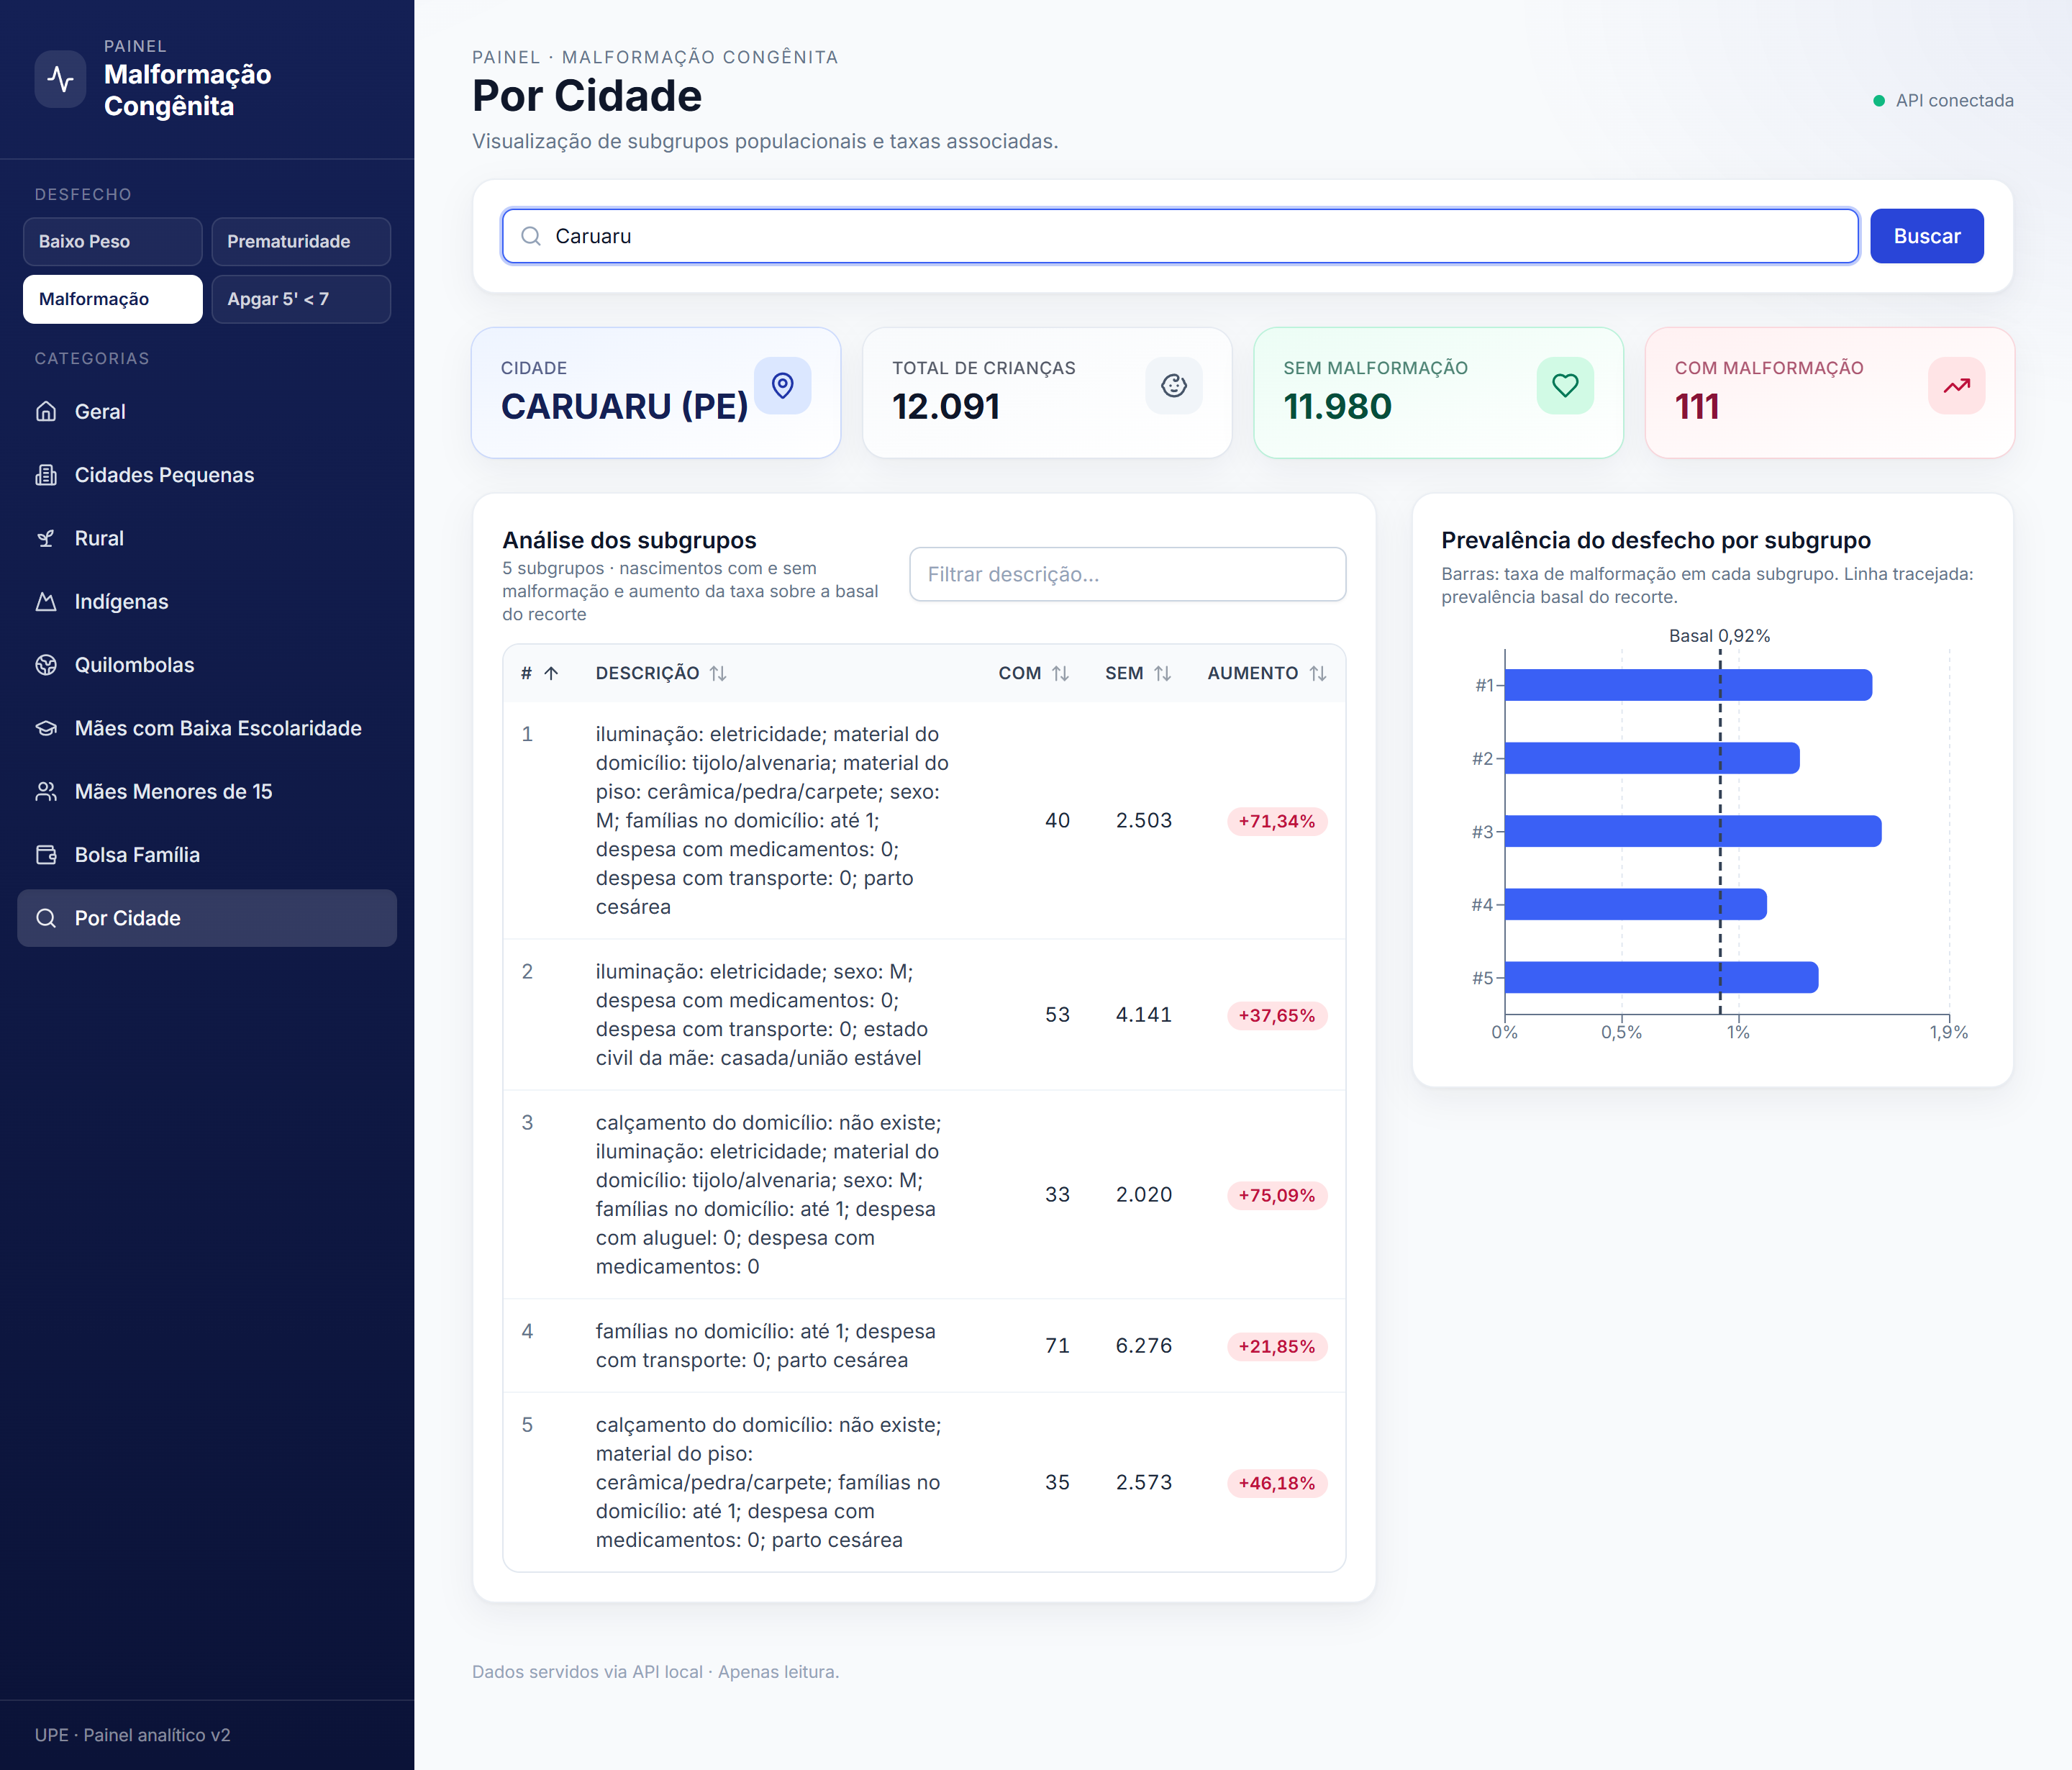
\includegraphics[width=\textwidth]{painel-caruaru}
\caption{Painel de visualização: subgrupos de malformação congênita no município de Caruaru (PE).}\label{fig:painel-caruaru}
\end{figure}

A navegação é feita por dois seletores, na barra lateral. O primeiro escolhe o desfecho (baixo peso, prematuridade, malformação ou Apgar no quinto minuto inferior a 7); o segundo escolhe a população, entre o recorte geral, os sete segmentos vulneráveis e a busca por município. Feita a escolha, o topo da tela resume a população selecionada em quatro indicadores: o nome do recorte, o total de nascimentos e quantos deles apresentaram ou não o desfecho. Em Caruaru, foram 12.091 nascimentos, dos quais 111 com malformação congênita, o que corresponde a uma prevalência basal de 0,92\%.

Abaixo dos indicadores, a tabela de análise lista os cinco subgrupos retornados para aquela população, numerados na ordem do SSDP+, da mesma forma que nas tabelas desta seção. Para cada regra, informa o número de nascimentos com e sem o desfecho e o aumento da taxa em relação à prevalência basal do recorte, que corresponde ao \emph{lift} menos um, expresso em porcentagem. A tabela pode ser ordenada por qualquer coluna e filtrada por texto, de modo que o usuário localize, por exemplo, todas as regras que envolvem o tipo de parto. Ao lado, um gráfico de barras mostra a prevalência do desfecho em cada subgrupo, com uma linha tracejada na prevalência basal do recorte: quanto mais a barra ultrapassa a linha, maior o \emph{lift} do subgrupo.

O exemplo de Caruaru reproduz, em escala municipal, o padrão observado na malformação congênita em todo o país, associado ao parto cesáreo, ao sexo masculino e a melhores condições de moradia. O parto cesáreo aparece em três das cinco regras (1, 4 e 5), o sexo masculino em outras três (1, 2 e 3), e itens como iluminação elétrica, domicílio de tijolo ou alvenaria e uma única família no domicílio se repetem entre elas. O subgrupo de maior risco (3) reúne ausência de calçamento, iluminação elétrica, domicílio de tijolo ou alvenaria, sexo masculino, uma única família no domicílio e despesas nulas com aluguel e medicamentos: são 2.053 nascimentos, 33 deles com malformação, o que equivale a uma prevalência de 1,61\%, 75\% acima da basal do município (\emph{lift} de 1,75). O subgrupo 1, com parto cesáreo e sexo masculino entre os seus itens, vem em seguida (71\% acima da basal), e a regra mais abrangente (4), com 6.347 nascimentos, combina parto cesáreo, uma única família no domicílio e despesa nula com transporte (22\% acima da basal). Assim, um gestor municipal pode identificar, em uma única consulta, os grupos em que a ocorrência do desfecho se concentra no seu território.
